\documentclass[dvisvgm]{standalone}
\usepackage{tikz}
\usepackage{pgfplots}

\begin{document}
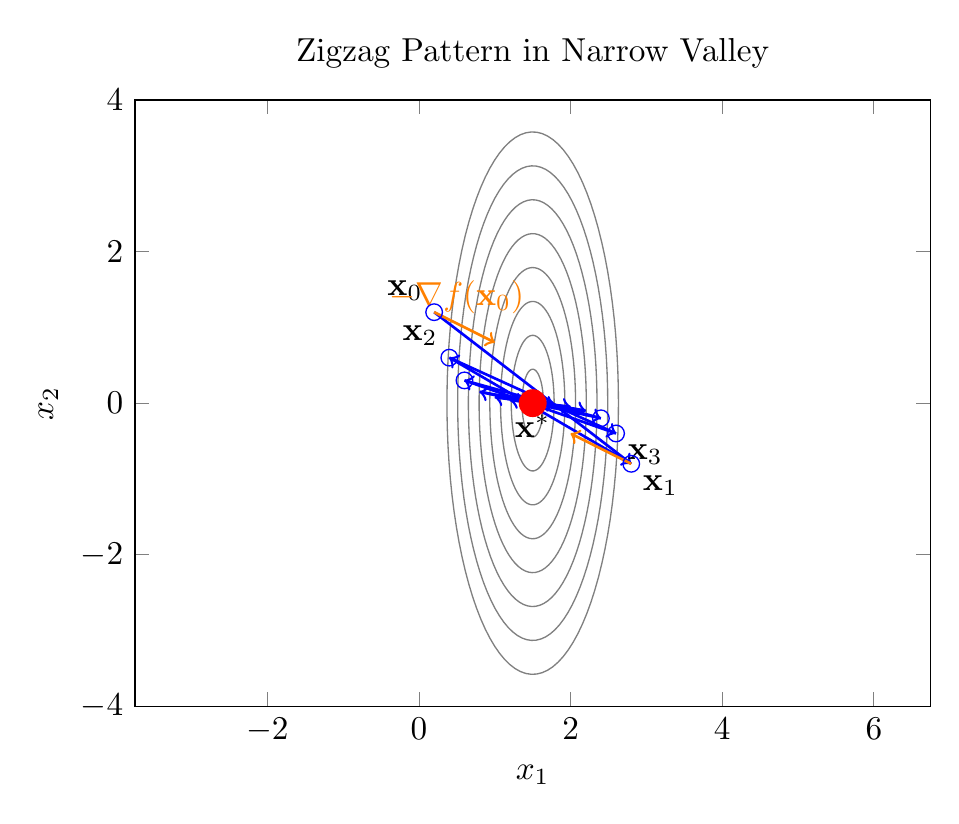
\begin{tikzpicture}[scale=1.2]
    \begin{axis}[
        width=10cm,
        height=8cm,
        xlabel={$x_1$},
        ylabel={$x_2$},
        grid=none,
        axis equal,
        xmin=-1, xmax=4,
        ymin=-4, ymax=4,
        title={Zigzag Pattern in Narrow Valley}
    ]
    
    % Draw elongated contour lines (poorly conditioned)
    \foreach \level in {0.2, 0.8, 1.8, 3.2, 5, 7.2, 9.8, 12.8}
    {
        \addplot[gray, thin, domain=0:360, samples=100] 
            ({1.5 + sqrt(\level/10)*cos(x)}, {sqrt(\level)*sin(x)});
    }
    
    % Mark the minimum
    \addplot[red, mark=*, mark size=4pt, only marks] coordinates {(1.5, 0)};
    \node at (axis cs:1.5,0) [below] {$\mathbf{x}^*$};
    
    % Zigzag trajectory points
    \coordinate (z0) at (axis cs:0.2, 1.2);
    \coordinate (z1) at (axis cs:2.8, -0.8);
    \coordinate (z2) at (axis cs:0.4, 0.6);
    \coordinate (z3) at (axis cs:2.6, -0.4);
    \coordinate (z4) at (axis cs:0.6, 0.3);
    \coordinate (z5) at (axis cs:2.4, -0.2);
    \coordinate (z6) at (axis cs:0.8, 0.15);
    \coordinate (z7) at (axis cs:2.2, -0.1);
    \coordinate (z8) at (axis cs:1.0, 0.08);
    \coordinate (z9) at (axis cs:2.0, -0.05);
    \coordinate (z10) at (axis cs:1.2, 0.04);
    \coordinate (z11) at (axis cs:1.8, -0.02);
    \coordinate (z12) at (axis cs:1.4, 0.01);
    \coordinate (z13) at (axis cs:1.5, 0);
    
    % Draw zigzag trajectory
    \draw[->, thick, blue] (z0) -- (z1);
    \draw[->, thick, blue] (z1) -- (z2);
    \draw[->, thick, blue] (z2) -- (z3);
    \draw[->, thick, blue] (z3) -- (z4);
    \draw[->, thick, blue] (z4) -- (z5);
    \draw[->, thick, blue] (z5) -- (z6);
    \draw[->, thick, blue] (z6) -- (z7);
    \draw[->, thick, blue] (z7) -- (z8);
    \draw[->, thick, blue] (z8) -- (z9);
    \draw[->, thick, blue] (z9) -- (z10);
    \draw[->, thick, blue] (z10) -- (z11);
    \draw[->, thick, blue] (z11) -- (z12);
    \draw[->, thick, blue] (z12) -- (z13);
    
    % Mark key iteration points
    \addplot[blue, mark=o, mark size=2.5pt, only marks] coordinates 
        {(0.2, 1.2) (2.8, -0.8) (0.4, 0.6) (2.6, -0.4) (0.6, 0.3) (2.4, -0.2)};
    
    % Add labels
    \node at (axis cs:0.2, 1.2) [above left] {$\mathbf{x}_0$};
    \node at (axis cs:2.8, -0.8) [below right] {$\mathbf{x}_1$};
    \node at (axis cs:0.4, 0.6) [above left] {$\mathbf{x}_2$};
    \node at (axis cs:2.6, -0.4) [below right] {$\mathbf{x}_3$};
    
    % Add some gradient vectors showing perpendicular directions
    \draw[->, thick, orange] (axis cs:0.2, 1.2) -- (axis cs:1.0, 0.8);
    \draw[->, thick, orange] (axis cs:2.8, -0.8) -- (axis cs:2.0, -0.4);
    \node at (axis cs:0.5, 1.4) [orange ] {$-\nabla f(\mathbf{x}_0)$};
    
    
    \end{axis}
\end{tikzpicture}
\end{document}
